\section{Normalization and Feature Processing}

\paragraph{Soil Properties:} 
Soil variables were normalized using property-specific transformations:
\begin{itemize}
    \item \textbf{Texture (COARSE, SAND, SILT, CLAY):} Min-Max scaling to range [0,1].
    \item \textbf{Density and pH:} Robust scaling for densities, Min-Max for pH.
    \item \textbf{Organic Matter and Nutrients:} Log-transform followed by robust scaling for organic carbon; log + standard scaling for total nitrogen; Min-Max for total carbon equivalents.
    \item \textbf{Cation Exchange and Fertility:} Robust scaling for CEC\_SOIL, CEC\_EFF, TEB; Min-Max for CEC\_CLAY, BSAT.
    \item \textbf{Salinity and Saturation:} Log-transform followed by robust scaling for ALUM\_SAT, ESP, GYPSUM, ELEC\_COND.
\end{itemize}

\subsection{Visualization of Normalization Effects}
The distributions of selected soil properties before and after normalization were compared to ensure consistency and scaling effectiveness.

\begin{figure}[H]
    \centering
    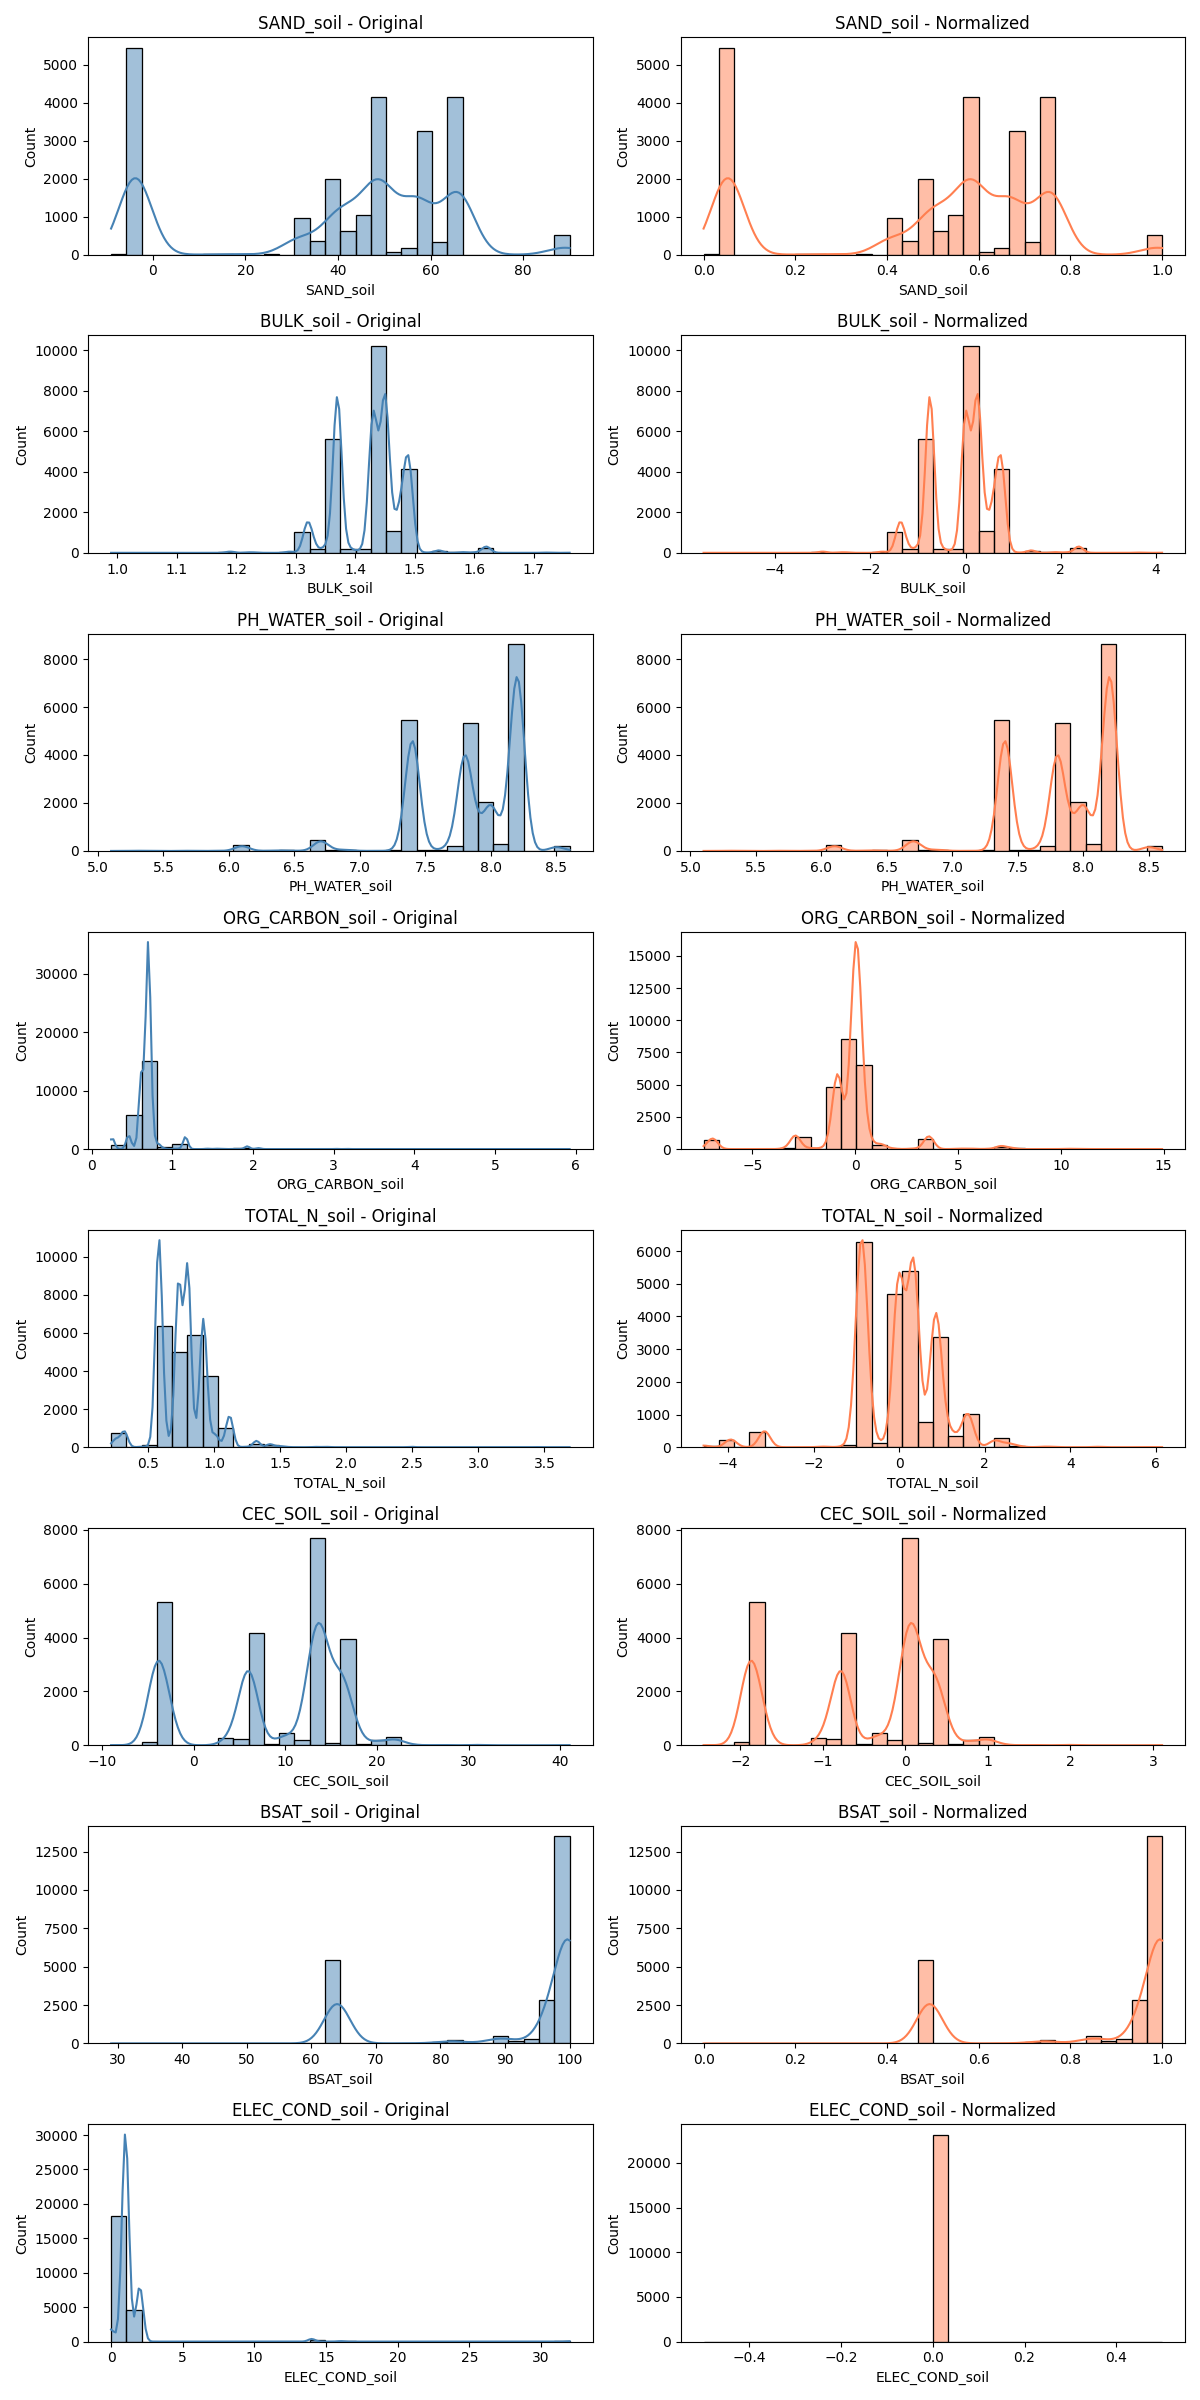
\includegraphics[width=0.6\textwidth]{images/MergedPreprocess/soil_normalization_comparison.png}
    \caption{Comparison of soil property distributions before and after normalization.}
    \label{fig:soil_normalization}
\end{figure}


\paragraph{Climate Features:} 
Temperature features were standardized (z-score), while precipitation features were log-transformed.

\paragraph{Elevation:} 
Standard scaling was applied to the elevation variable.

\paragraph{Landcover:} 
The original land cover codes (\texttt{lcccode}) were transformed into higher-level categories (\texttt{lcc\_highlevel}) to simplify the representation of land types. 
For instance:
\begin{itemize}
    \item Multiple codes corresponding to water-related classes (e.g., 7001, 8001) were grouped as ``Water bodies''.
    \item Forest-related codes (e.g., 21497-121340) were grouped as ``Forests''.
\end{itemize}
This high-level categorization reduces the number of classes and improves model interpretability, while preserving the main land cover distinctions.

\begin{table}[H]
    \centering
    \caption{Example of Landcover Transformation from \texttt{lcccode} to \texttt{lcc\_highlevel}}
    \label{tab:landcover_highlevel}
    \begin{tabular}{cc}
        \toprule
        \textbf{lcccode} & \textbf{lcc\_highlevel} \\
        \midrule
        7001 // 8001      & Water bodies \\
        7001 // 8001      & Water bodies \\
        7001 // 8001      & Water bodies \\
        21497-121340      & Forests \\
        7001 // 8001      & Water bodies \\
        \bottomrule
    \end{tabular}
\end{table}


\subsection{Saving the Normalized Data}
The final normalized dataset (\texttt{X\_train}) was saved in Parquet format for subsequent modeling steps.
